% Created by tikzDevice version 0.10.1 on 2017-10-23 14:30:15
% !TEX encoding = UTF-8 Unicode
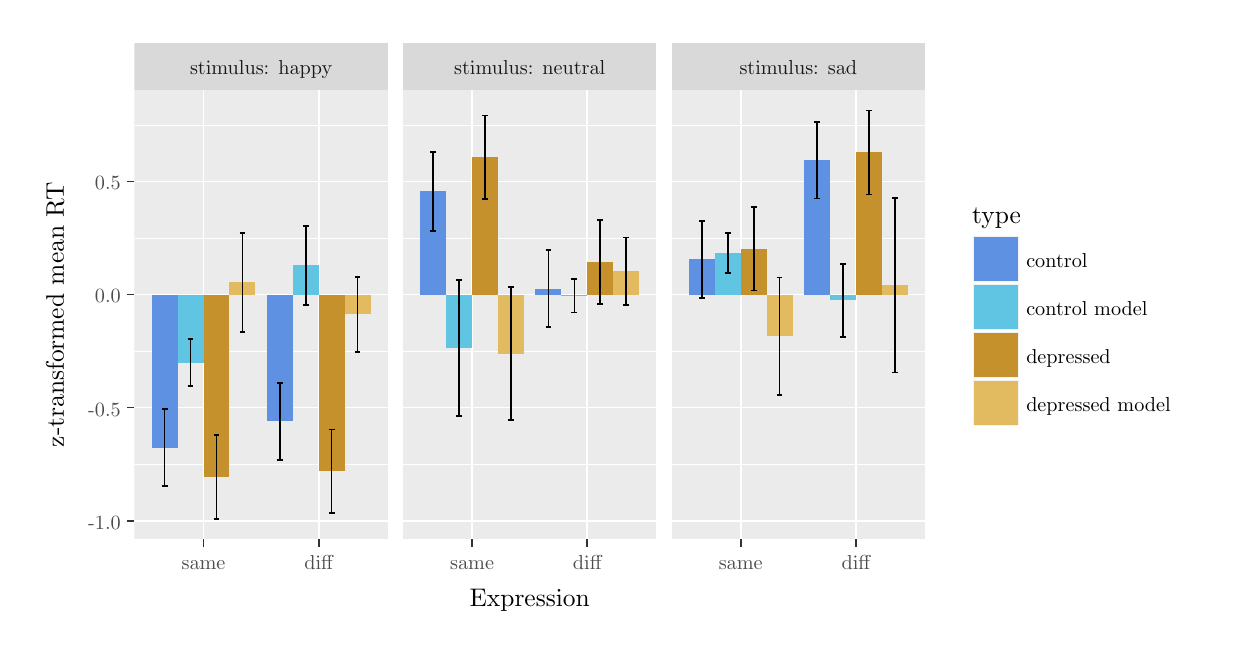
\begin{tikzpicture}[x=1pt,y=1pt]
\definecolor{fillColor}{RGB}{255,255,255}
\path[use as bounding box,fill=fillColor,fill opacity=0.00] (0,0) rectangle (433.62,216.81);
\begin{scope}
\path[clip] (  0.00,  0.00) rectangle (433.62,216.81);
\definecolor{drawColor}{RGB}{255,255,255}
\definecolor{fillColor}{RGB}{255,255,255}

\path[draw=drawColor,line width= 0.6pt,line join=round,line cap=round,fill=fillColor] ( -0.00,  0.00) rectangle (433.62,216.81);
\end{scope}
\begin{scope}
\path[clip] ( 38.57, 31.92) rectangle (130.13,194.25);
\definecolor{fillColor}{gray}{0.92}

\path[fill=fillColor] ( 38.57, 31.92) rectangle (130.13,194.25);
\definecolor{drawColor}{RGB}{255,255,255}

\path[draw=drawColor,line width= 0.3pt,line join=round] ( 38.57, 59.08) --
	(130.13, 59.08);

\path[draw=drawColor,line width= 0.3pt,line join=round] ( 38.57, 99.94) --
	(130.13, 99.94);

\path[draw=drawColor,line width= 0.3pt,line join=round] ( 38.57,140.80) --
	(130.13,140.80);

\path[draw=drawColor,line width= 0.3pt,line join=round] ( 38.57,181.65) --
	(130.13,181.65);

\path[draw=drawColor,line width= 0.6pt,line join=round] ( 38.57, 38.65) --
	(130.13, 38.65);

\path[draw=drawColor,line width= 0.6pt,line join=round] ( 38.57, 79.51) --
	(130.13, 79.51);

\path[draw=drawColor,line width= 0.6pt,line join=round] ( 38.57,120.37) --
	(130.13,120.37);

\path[draw=drawColor,line width= 0.6pt,line join=round] ( 38.57,161.23) --
	(130.13,161.23);

\path[draw=drawColor,line width= 0.6pt,line join=round] ( 63.54, 31.92) --
	( 63.54,194.25);

\path[draw=drawColor,line width= 0.6pt,line join=round] (105.16, 31.92) --
	(105.16,194.25);
\definecolor{fillColor}{RGB}{226,186,95}

\path[fill=fillColor] ( 72.91,120.37) rectangle ( 82.27,124.80);
\definecolor{fillColor}{RGB}{196,145,45}

\path[fill=fillColor] ( 63.54, 54.41) rectangle ( 72.91,120.37);
\definecolor{fillColor}{RGB}{95,197,226}

\path[fill=fillColor] ( 54.18, 95.80) rectangle ( 63.54,120.37);
\definecolor{fillColor}{RGB}{95,145,226}

\path[fill=fillColor] ( 44.81, 65.08) rectangle ( 54.18,120.37);
\definecolor{fillColor}{RGB}{226,186,95}

\path[fill=fillColor] (114.52,113.21) rectangle (123.89,120.37);
\definecolor{fillColor}{RGB}{196,145,45}

\path[fill=fillColor] (105.16, 56.55) rectangle (114.52,120.37);
\definecolor{fillColor}{RGB}{95,197,226}

\path[fill=fillColor] ( 95.80,120.37) rectangle (105.16,130.96);
\definecolor{fillColor}{RGB}{95,145,226}

\path[fill=fillColor] ( 86.43, 74.57) rectangle ( 95.80,120.37);
\definecolor{drawColor}{RGB}{0,0,0}

\path[draw=drawColor,line width= 0.6pt,line join=round] ( 76.55,142.67) --
	( 78.63,142.67);

\path[draw=drawColor,line width= 0.6pt,line join=round] ( 77.59,142.67) --
	( 77.59,106.93);

\path[draw=drawColor,line width= 0.6pt,line join=round] ( 76.55,106.93) --
	( 78.63,106.93);

\path[draw=drawColor,line width= 0.6pt,line join=round] ( 67.18, 69.53) --
	( 69.26, 69.53);

\path[draw=drawColor,line width= 0.6pt,line join=round] ( 68.22, 69.53) --
	( 68.22, 39.30);

\path[draw=drawColor,line width= 0.6pt,line join=round] ( 67.18, 39.30) --
	( 69.26, 39.30);

\path[draw=drawColor,line width= 0.6pt,line join=round] ( 57.82,104.37) --
	( 59.90,104.37);

\path[draw=drawColor,line width= 0.6pt,line join=round] ( 58.86,104.37) --
	( 58.86, 87.22);

\path[draw=drawColor,line width= 0.6pt,line join=round] ( 57.82, 87.22) --
	( 59.90, 87.22);

\path[draw=drawColor,line width= 0.6pt,line join=round] ( 48.46, 78.96) --
	( 50.54, 78.96);

\path[draw=drawColor,line width= 0.6pt,line join=round] ( 49.50, 78.96) --
	( 49.50, 51.19);

\path[draw=drawColor,line width= 0.6pt,line join=round] ( 48.46, 51.19) --
	( 50.54, 51.19);

\path[draw=drawColor,line width= 0.6pt,line join=round] (118.17,126.80) --
	(120.25,126.80);

\path[draw=drawColor,line width= 0.6pt,line join=round] (119.21,126.80) --
	(119.21, 99.61);

\path[draw=drawColor,line width= 0.6pt,line join=round] (118.17, 99.61) --
	(120.25, 99.61);

\path[draw=drawColor,line width= 0.6pt,line join=round] (108.80, 71.66) --
	(110.88, 71.66);

\path[draw=drawColor,line width= 0.6pt,line join=round] (109.84, 71.66) --
	(109.84, 41.43);

\path[draw=drawColor,line width= 0.6pt,line join=round] (108.80, 41.43) --
	(110.88, 41.43);

\path[draw=drawColor,line width= 0.6pt,line join=round] ( 99.44,145.24) --
	(101.52,145.24);

\path[draw=drawColor,line width= 0.6pt,line join=round] (100.48,145.24) --
	(100.48,116.68);

\path[draw=drawColor,line width= 0.6pt,line join=round] ( 99.44,116.68) --
	(101.52,116.68);

\path[draw=drawColor,line width= 0.6pt,line join=round] ( 90.07, 88.49) --
	( 92.15, 88.49);

\path[draw=drawColor,line width= 0.6pt,line join=round] ( 91.11, 88.49) --
	( 91.11, 60.65);

\path[draw=drawColor,line width= 0.6pt,line join=round] ( 90.07, 60.65) --
	( 92.15, 60.65);
\end{scope}
\begin{scope}
\path[clip] (135.63, 31.92) rectangle (227.19,194.25);
\definecolor{fillColor}{gray}{0.92}

\path[fill=fillColor] (135.63, 31.92) rectangle (227.19,194.25);
\definecolor{drawColor}{RGB}{255,255,255}

\path[draw=drawColor,line width= 0.3pt,line join=round] (135.63, 59.08) --
	(227.19, 59.08);

\path[draw=drawColor,line width= 0.3pt,line join=round] (135.63, 99.94) --
	(227.19, 99.94);

\path[draw=drawColor,line width= 0.3pt,line join=round] (135.63,140.80) --
	(227.19,140.80);

\path[draw=drawColor,line width= 0.3pt,line join=round] (135.63,181.65) --
	(227.19,181.65);

\path[draw=drawColor,line width= 0.6pt,line join=round] (135.63, 38.65) --
	(227.19, 38.65);

\path[draw=drawColor,line width= 0.6pt,line join=round] (135.63, 79.51) --
	(227.19, 79.51);

\path[draw=drawColor,line width= 0.6pt,line join=round] (135.63,120.37) --
	(227.19,120.37);

\path[draw=drawColor,line width= 0.6pt,line join=round] (135.63,161.23) --
	(227.19,161.23);

\path[draw=drawColor,line width= 0.6pt,line join=round] (160.60, 31.92) --
	(160.60,194.25);

\path[draw=drawColor,line width= 0.6pt,line join=round] (202.22, 31.92) --
	(202.22,194.25);
\definecolor{fillColor}{RGB}{226,186,95}

\path[fill=fillColor] (169.97, 98.99) rectangle (179.33,120.37);
\definecolor{fillColor}{RGB}{196,145,45}

\path[fill=fillColor] (160.60,120.37) rectangle (169.97,169.91);
\definecolor{fillColor}{RGB}{95,197,226}

\path[fill=fillColor] (151.24,101.09) rectangle (160.60,120.37);
\definecolor{fillColor}{RGB}{95,145,226}

\path[fill=fillColor] (141.87,120.37) rectangle (151.24,157.64);
\definecolor{fillColor}{RGB}{226,186,95}

\path[fill=fillColor] (211.59,120.37) rectangle (220.95,128.76);
\definecolor{fillColor}{RGB}{196,145,45}

\path[fill=fillColor] (202.22,120.37) rectangle (211.59,132.13);
\definecolor{fillColor}{RGB}{95,197,226}

\path[fill=fillColor] (192.86,119.87) rectangle (202.22,120.37);
\definecolor{fillColor}{RGB}{95,145,226}

\path[fill=fillColor] (183.49,120.37) rectangle (192.86,122.50);
\definecolor{drawColor}{RGB}{0,0,0}

\path[draw=drawColor,line width= 0.6pt,line join=round] (173.61,123.04) --
	(175.69,123.04);

\path[draw=drawColor,line width= 0.6pt,line join=round] (174.65,123.04) --
	(174.65, 74.94);

\path[draw=drawColor,line width= 0.6pt,line join=round] (173.61, 74.94) --
	(175.69, 74.94);

\path[draw=drawColor,line width= 0.6pt,line join=round] (164.24,185.03) --
	(166.33,185.03);

\path[draw=drawColor,line width= 0.6pt,line join=round] (165.28,185.03) --
	(165.28,154.80);

\path[draw=drawColor,line width= 0.6pt,line join=round] (164.24,154.80) --
	(166.33,154.80);

\path[draw=drawColor,line width= 0.6pt,line join=round] (154.88,125.58) --
	(156.96,125.58);

\path[draw=drawColor,line width= 0.6pt,line join=round] (155.92,125.58) --
	(155.92, 76.60);

\path[draw=drawColor,line width= 0.6pt,line join=round] (154.88, 76.60) --
	(156.96, 76.60);

\path[draw=drawColor,line width= 0.6pt,line join=round] (145.52,171.89) --
	(147.60,171.89);

\path[draw=drawColor,line width= 0.6pt,line join=round] (146.56,171.89) --
	(146.56,143.40);

\path[draw=drawColor,line width= 0.6pt,line join=round] (145.52,143.40) --
	(147.60,143.40);

\path[draw=drawColor,line width= 0.6pt,line join=round] (215.23,141.01) --
	(217.31,141.01);

\path[draw=drawColor,line width= 0.6pt,line join=round] (216.27,141.01) --
	(216.27,116.51);

\path[draw=drawColor,line width= 0.6pt,line join=round] (215.23,116.51) --
	(217.31,116.51);

\path[draw=drawColor,line width= 0.6pt,line join=round] (205.86,147.27) --
	(207.94,147.27);

\path[draw=drawColor,line width= 0.6pt,line join=round] (206.90,147.27) --
	(206.90,116.98);

\path[draw=drawColor,line width= 0.6pt,line join=round] (205.86,116.98) --
	(207.94,116.98);

\path[draw=drawColor,line width= 0.6pt,line join=round] (196.50,125.88) --
	(198.58,125.88);

\path[draw=drawColor,line width= 0.6pt,line join=round] (197.54,125.88) --
	(197.54,113.86);

\path[draw=drawColor,line width= 0.6pt,line join=round] (196.50,113.86) --
	(198.58,113.86);

\path[draw=drawColor,line width= 0.6pt,line join=round] (187.13,136.39) --
	(189.22,136.39);

\path[draw=drawColor,line width= 0.6pt,line join=round] (188.18,136.39) --
	(188.18,108.61);

\path[draw=drawColor,line width= 0.6pt,line join=round] (187.13,108.61) --
	(189.22,108.61);
\end{scope}
\begin{scope}
\path[clip] (232.69, 31.92) rectangle (324.25,194.25);
\definecolor{fillColor}{gray}{0.92}

\path[fill=fillColor] (232.69, 31.92) rectangle (324.25,194.25);
\definecolor{drawColor}{RGB}{255,255,255}

\path[draw=drawColor,line width= 0.3pt,line join=round] (232.69, 59.08) --
	(324.25, 59.08);

\path[draw=drawColor,line width= 0.3pt,line join=round] (232.69, 99.94) --
	(324.25, 99.94);

\path[draw=drawColor,line width= 0.3pt,line join=round] (232.69,140.80) --
	(324.25,140.80);

\path[draw=drawColor,line width= 0.3pt,line join=round] (232.69,181.65) --
	(324.25,181.65);

\path[draw=drawColor,line width= 0.6pt,line join=round] (232.69, 38.65) --
	(324.25, 38.65);

\path[draw=drawColor,line width= 0.6pt,line join=round] (232.69, 79.51) --
	(324.25, 79.51);

\path[draw=drawColor,line width= 0.6pt,line join=round] (232.69,120.37) --
	(324.25,120.37);

\path[draw=drawColor,line width= 0.6pt,line join=round] (232.69,161.23) --
	(324.25,161.23);

\path[draw=drawColor,line width= 0.6pt,line join=round] (257.66, 31.92) --
	(257.66,194.25);

\path[draw=drawColor,line width= 0.6pt,line join=round] (299.28, 31.92) --
	(299.28,194.25);
\definecolor{fillColor}{RGB}{226,186,95}

\path[fill=fillColor] (267.03,105.31) rectangle (276.39,120.37);
\definecolor{fillColor}{RGB}{196,145,45}

\path[fill=fillColor] (257.66,120.37) rectangle (267.03,136.91);
\definecolor{fillColor}{RGB}{95,197,226}

\path[fill=fillColor] (248.30,120.37) rectangle (257.66,135.36);
\definecolor{fillColor}{RGB}{95,145,226}

\path[fill=fillColor] (238.94,120.37) rectangle (248.30,133.10);
\definecolor{fillColor}{RGB}{226,186,95}

\path[fill=fillColor] (308.65,120.37) rectangle (318.01,123.77);
\definecolor{fillColor}{RGB}{196,145,45}

\path[fill=fillColor] (299.28,120.37) rectangle (308.65,171.72);
\definecolor{fillColor}{RGB}{95,197,226}

\path[fill=fillColor] (289.92,118.27) rectangle (299.28,120.37);
\definecolor{fillColor}{RGB}{95,145,226}

\path[fill=fillColor] (280.55,120.37) rectangle (289.92,168.95);
\definecolor{drawColor}{RGB}{0,0,0}

\path[draw=drawColor,line width= 0.6pt,line join=round] (270.67,126.53) --
	(272.75,126.53);

\path[draw=drawColor,line width= 0.6pt,line join=round] (271.71,126.53) --
	(271.71, 84.08);

\path[draw=drawColor,line width= 0.6pt,line join=round] (270.67, 84.08) --
	(272.75, 84.08);

\path[draw=drawColor,line width= 0.6pt,line join=round] (261.31,152.02) --
	(263.39,152.02);

\path[draw=drawColor,line width= 0.6pt,line join=round] (262.35,152.02) --
	(262.35,121.79);

\path[draw=drawColor,line width= 0.6pt,line join=round] (261.31,121.79) --
	(263.39,121.79);

\path[draw=drawColor,line width= 0.6pt,line join=round] (251.94,142.66) --
	(254.02,142.66);

\path[draw=drawColor,line width= 0.6pt,line join=round] (252.98,142.66) --
	(252.98,128.06);

\path[draw=drawColor,line width= 0.6pt,line join=round] (251.94,128.06) --
	(254.02,128.06);

\path[draw=drawColor,line width= 0.6pt,line join=round] (242.58,146.99) --
	(244.66,146.99);

\path[draw=drawColor,line width= 0.6pt,line join=round] (243.62,146.99) --
	(243.62,119.21);

\path[draw=drawColor,line width= 0.6pt,line join=round] (242.58,119.21) --
	(244.66,119.21);

\path[draw=drawColor,line width= 0.6pt,line join=round] (312.29,155.33) --
	(314.37,155.33);

\path[draw=drawColor,line width= 0.6pt,line join=round] (313.33,155.33) --
	(313.33, 92.21);

\path[draw=drawColor,line width= 0.6pt,line join=round] (312.29, 92.21) --
	(314.37, 92.21);

\path[draw=drawColor,line width= 0.6pt,line join=round] (302.92,186.87) --
	(305.00,186.87);

\path[draw=drawColor,line width= 0.6pt,line join=round] (303.96,186.87) --
	(303.96,156.58);

\path[draw=drawColor,line width= 0.6pt,line join=round] (302.92,156.58) --
	(305.00,156.58);

\path[draw=drawColor,line width= 0.6pt,line join=round] (293.56,131.50) --
	(295.64,131.50);

\path[draw=drawColor,line width= 0.6pt,line join=round] (294.60,131.50) --
	(294.60,105.05);

\path[draw=drawColor,line width= 0.6pt,line join=round] (293.56,105.05) --
	(295.64,105.05);

\path[draw=drawColor,line width= 0.6pt,line join=round] (284.20,182.84) --
	(286.28,182.84);

\path[draw=drawColor,line width= 0.6pt,line join=round] (285.24,182.84) --
	(285.24,155.06);

\path[draw=drawColor,line width= 0.6pt,line join=round] (284.20,155.06) --
	(286.28,155.06);
\end{scope}
\begin{scope}
\path[clip] ( 38.57,194.25) rectangle (130.13,211.31);
\definecolor{fillColor}{gray}{0.85}

\path[fill=fillColor] ( 38.57,194.25) rectangle (130.13,211.31);
\definecolor{drawColor}{gray}{0.10}

\node[text=drawColor,anchor=base,inner sep=0pt, outer sep=0pt, scale=  0.73] at ( 84.35,199.75) {stimulus: happy};
\end{scope}
\begin{scope}
\path[clip] (135.63,194.25) rectangle (227.19,211.31);
\definecolor{fillColor}{gray}{0.85}

\path[fill=fillColor] (135.63,194.25) rectangle (227.19,211.31);
\definecolor{drawColor}{gray}{0.10}

\node[text=drawColor,anchor=base,inner sep=0pt, outer sep=0pt, scale=  0.73] at (181.41,199.75) {stimulus: neutral};
\end{scope}
\begin{scope}
\path[clip] (232.69,194.25) rectangle (324.25,211.31);
\definecolor{fillColor}{gray}{0.85}

\path[fill=fillColor] (232.69,194.25) rectangle (324.25,211.31);
\definecolor{drawColor}{gray}{0.10}

\node[text=drawColor,anchor=base,inner sep=0pt, outer sep=0pt, scale=  0.73] at (278.47,199.75) {stimulus: sad};
\end{scope}
\begin{scope}
\path[clip] (  0.00,  0.00) rectangle (433.62,216.81);
\definecolor{drawColor}{gray}{0.20}

\path[draw=drawColor,line width= 0.6pt,line join=round] ( 63.54, 29.17) --
	( 63.54, 31.92);

\path[draw=drawColor,line width= 0.6pt,line join=round] (105.16, 29.17) --
	(105.16, 31.92);
\end{scope}
\begin{scope}
\path[clip] (  0.00,  0.00) rectangle (433.62,216.81);
\definecolor{drawColor}{gray}{0.30}

\node[text=drawColor,anchor=base,inner sep=0pt, outer sep=0pt, scale=  0.73] at ( 63.54, 20.91) {same};

\node[text=drawColor,anchor=base,inner sep=0pt, outer sep=0pt, scale=  0.73] at (105.16, 20.91) {diff};
\end{scope}
\begin{scope}
\path[clip] (  0.00,  0.00) rectangle (433.62,216.81);
\definecolor{drawColor}{gray}{0.20}

\path[draw=drawColor,line width= 0.6pt,line join=round] (160.60, 29.17) --
	(160.60, 31.92);

\path[draw=drawColor,line width= 0.6pt,line join=round] (202.22, 29.17) --
	(202.22, 31.92);
\end{scope}
\begin{scope}
\path[clip] (  0.00,  0.00) rectangle (433.62,216.81);
\definecolor{drawColor}{gray}{0.30}

\node[text=drawColor,anchor=base,inner sep=0pt, outer sep=0pt, scale=  0.73] at (160.60, 20.91) {same};

\node[text=drawColor,anchor=base,inner sep=0pt, outer sep=0pt, scale=  0.73] at (202.22, 20.91) {diff};
\end{scope}
\begin{scope}
\path[clip] (  0.00,  0.00) rectangle (433.62,216.81);
\definecolor{drawColor}{gray}{0.20}

\path[draw=drawColor,line width= 0.6pt,line join=round] (257.66, 29.17) --
	(257.66, 31.92);

\path[draw=drawColor,line width= 0.6pt,line join=round] (299.28, 29.17) --
	(299.28, 31.92);
\end{scope}
\begin{scope}
\path[clip] (  0.00,  0.00) rectangle (433.62,216.81);
\definecolor{drawColor}{gray}{0.30}

\node[text=drawColor,anchor=base,inner sep=0pt, outer sep=0pt, scale=  0.73] at (257.66, 20.91) {same};

\node[text=drawColor,anchor=base,inner sep=0pt, outer sep=0pt, scale=  0.73] at (299.28, 20.91) {diff};
\end{scope}
\begin{scope}
\path[clip] (  0.00,  0.00) rectangle (433.62,216.81);
\definecolor{drawColor}{gray}{0.30}

\node[text=drawColor,anchor=base east,inner sep=0pt, outer sep=0pt, scale=  0.73] at ( 33.62, 35.62) {-1.0};

\node[text=drawColor,anchor=base east,inner sep=0pt, outer sep=0pt, scale=  0.73] at ( 33.62, 76.48) {-0.5};

\node[text=drawColor,anchor=base east,inner sep=0pt, outer sep=0pt, scale=  0.73] at ( 33.62,117.34) {0.0};

\node[text=drawColor,anchor=base east,inner sep=0pt, outer sep=0pt, scale=  0.73] at ( 33.62,158.20) {0.5};
\end{scope}
\begin{scope}
\path[clip] (  0.00,  0.00) rectangle (433.62,216.81);
\definecolor{drawColor}{gray}{0.20}

\path[draw=drawColor,line width= 0.6pt,line join=round] ( 35.82, 38.65) --
	( 38.57, 38.65);

\path[draw=drawColor,line width= 0.6pt,line join=round] ( 35.82, 79.51) --
	( 38.57, 79.51);

\path[draw=drawColor,line width= 0.6pt,line join=round] ( 35.82,120.37) --
	( 38.57,120.37);

\path[draw=drawColor,line width= 0.6pt,line join=round] ( 35.82,161.23) --
	( 38.57,161.23);
\end{scope}
\begin{scope}
\path[clip] (  0.00,  0.00) rectangle (433.62,216.81);
\definecolor{drawColor}{RGB}{0,0,0}

\node[text=drawColor,anchor=base,inner sep=0pt, outer sep=0pt, scale=  0.92] at (181.41,  7.83) {Expression};
\end{scope}
\begin{scope}
\path[clip] (  0.00,  0.00) rectangle (433.62,216.81);
\definecolor{drawColor}{RGB}{0,0,0}

\node[text=drawColor,rotate= 90.00,anchor=base,inner sep=0pt, outer sep=0pt, scale=  0.92] at ( 13.08,113.08) {z-transformed mean RT};
\end{scope}
\begin{scope}
\path[clip] (  0.00,  0.00) rectangle (433.62,216.81);
\definecolor{fillColor}{RGB}{255,255,255}

\path[fill=fillColor] (335.63, 66.75) rectangle (428.12,159.42);
\end{scope}
\begin{scope}
\path[clip] (  0.00,  0.00) rectangle (433.62,216.81);
\definecolor{drawColor}{RGB}{0,0,0}

\node[text=drawColor,anchor=base west,inner sep=0pt, outer sep=0pt, scale=  0.92] at (341.32,146.15) {type};
\end{scope}
\begin{scope}
\path[clip] (  0.00,  0.00) rectangle (433.62,216.81);
\definecolor{drawColor}{RGB}{255,255,255}
\definecolor{fillColor}{gray}{0.95}

\path[draw=drawColor,line width= 0.6pt,line join=round,line cap=round,fill=fillColor] (341.32,124.47) rectangle (358.67,141.82);
\end{scope}
\begin{scope}
\path[clip] (  0.00,  0.00) rectangle (433.62,216.81);
\definecolor{fillColor}{RGB}{95,145,226}

\path[fill=fillColor] (342.04,125.18) rectangle (357.96,141.11);
\end{scope}
\begin{scope}
\path[clip] (  0.00,  0.00) rectangle (433.62,216.81);
\definecolor{drawColor}{RGB}{255,255,255}
\definecolor{fillColor}{gray}{0.95}

\path[draw=drawColor,line width= 0.6pt,line join=round,line cap=round,fill=fillColor] (341.32,107.13) rectangle (358.67,124.47);
\end{scope}
\begin{scope}
\path[clip] (  0.00,  0.00) rectangle (433.62,216.81);
\definecolor{fillColor}{RGB}{95,197,226}

\path[fill=fillColor] (342.04,107.84) rectangle (357.96,123.76);
\end{scope}
\begin{scope}
\path[clip] (  0.00,  0.00) rectangle (433.62,216.81);
\definecolor{drawColor}{RGB}{255,255,255}
\definecolor{fillColor}{gray}{0.95}

\path[draw=drawColor,line width= 0.6pt,line join=round,line cap=round,fill=fillColor] (341.32, 89.78) rectangle (358.67,107.13);
\end{scope}
\begin{scope}
\path[clip] (  0.00,  0.00) rectangle (433.62,216.81);
\definecolor{fillColor}{RGB}{196,145,45}

\path[fill=fillColor] (342.04, 90.49) rectangle (357.96,106.42);
\end{scope}
\begin{scope}
\path[clip] (  0.00,  0.00) rectangle (433.62,216.81);
\definecolor{drawColor}{RGB}{255,255,255}
\definecolor{fillColor}{gray}{0.95}

\path[draw=drawColor,line width= 0.6pt,line join=round,line cap=round,fill=fillColor] (341.32, 72.44) rectangle (358.67, 89.78);
\end{scope}
\begin{scope}
\path[clip] (  0.00,  0.00) rectangle (433.62,216.81);
\definecolor{fillColor}{RGB}{226,186,95}

\path[fill=fillColor] (342.04, 73.15) rectangle (357.96, 89.07);
\end{scope}
\begin{scope}
\path[clip] (  0.00,  0.00) rectangle (433.62,216.81);
\definecolor{drawColor}{RGB}{0,0,0}

\node[text=drawColor,anchor=base west,inner sep=0pt, outer sep=0pt, scale=  0.73] at (360.84,130.12) {control};
\end{scope}
\begin{scope}
\path[clip] (  0.00,  0.00) rectangle (433.62,216.81);
\definecolor{drawColor}{RGB}{0,0,0}

\node[text=drawColor,anchor=base west,inner sep=0pt, outer sep=0pt, scale=  0.73] at (360.84,112.77) {control model};
\end{scope}
\begin{scope}
\path[clip] (  0.00,  0.00) rectangle (433.62,216.81);
\definecolor{drawColor}{RGB}{0,0,0}

\node[text=drawColor,anchor=base west,inner sep=0pt, outer sep=0pt, scale=  0.73] at (360.84, 95.43) {depressed};
\end{scope}
\begin{scope}
\path[clip] (  0.00,  0.00) rectangle (433.62,216.81);
\definecolor{drawColor}{RGB}{0,0,0}

\node[text=drawColor,anchor=base west,inner sep=0pt, outer sep=0pt, scale=  0.73] at (360.84, 78.08) {depressed model};
\end{scope}
\end{tikzpicture}
